\documentclass[twoside]{book}

% Packages required by doxygen
\usepackage{fixltx2e}
\usepackage{calc}
\usepackage{doxygen}
\usepackage[export]{adjustbox} % also loads graphicx
\usepackage{graphicx}
\usepackage[utf8]{inputenc}
\usepackage{makeidx}
\usepackage{multicol}
\usepackage{multirow}
\PassOptionsToPackage{warn}{textcomp}
\usepackage{textcomp}
\usepackage[nointegrals]{wasysym}
\usepackage[table]{xcolor}

% Font selection
\usepackage[T1]{fontenc}
\usepackage[scaled=.90]{helvet}
\usepackage{courier}
\usepackage{amssymb}
\usepackage{sectsty}
\renewcommand{\familydefault}{\sfdefault}
\allsectionsfont{%
  \fontseries{bc}\selectfont%
  \color{darkgray}%
}
\renewcommand{\DoxyLabelFont}{%
  \fontseries{bc}\selectfont%
  \color{darkgray}%
}
\newcommand{\+}{\discretionary{\mbox{\scriptsize$\hookleftarrow$}}{}{}}

% Page & text layout
\usepackage{geometry}
\geometry{%
  a4paper,%
  top=2.5cm,%
  bottom=2.5cm,%
  left=2.5cm,%
  right=2.5cm%
}
\tolerance=750
\hfuzz=15pt
\hbadness=750
\setlength{\emergencystretch}{15pt}
\setlength{\parindent}{0cm}
\setlength{\parskip}{3ex plus 2ex minus 2ex}
\makeatletter
\renewcommand{\paragraph}{%
  \@startsection{paragraph}{4}{0ex}{-1.0ex}{1.0ex}{%
    \normalfont\normalsize\bfseries\SS@parafont%
  }%
}
\renewcommand{\subparagraph}{%
  \@startsection{subparagraph}{5}{0ex}{-1.0ex}{1.0ex}{%
    \normalfont\normalsize\bfseries\SS@subparafont%
  }%
}
\makeatother

% Headers & footers
\usepackage{fancyhdr}
\pagestyle{fancyplain}
\fancyhead[LE]{\fancyplain{}{\bfseries\thepage}}
\fancyhead[CE]{\fancyplain{}{}}
\fancyhead[RE]{\fancyplain{}{\bfseries\leftmark}}
\fancyhead[LO]{\fancyplain{}{\bfseries\rightmark}}
\fancyhead[CO]{\fancyplain{}{}}
\fancyhead[RO]{\fancyplain{}{\bfseries\thepage}}
\fancyfoot[LE]{\fancyplain{}{}}
\fancyfoot[CE]{\fancyplain{}{}}
\fancyfoot[RE]{\fancyplain{}{\bfseries\scriptsize Generated by Doxygen }}
\fancyfoot[LO]{\fancyplain{}{\bfseries\scriptsize Generated by Doxygen }}
\fancyfoot[CO]{\fancyplain{}{}}
\fancyfoot[RO]{\fancyplain{}{}}
\renewcommand{\footrulewidth}{0.4pt}
\renewcommand{\chaptermark}[1]{%
  \markboth{#1}{}%
}
\renewcommand{\sectionmark}[1]{%
  \markright{\thesection\ #1}%
}

% Indices & bibliography
\usepackage{natbib}
\usepackage[titles]{tocloft}
\setcounter{tocdepth}{3}
\setcounter{secnumdepth}{5}
\makeindex

% Hyperlinks (required, but should be loaded last)
\usepackage{ifpdf}
\ifpdf
  \usepackage[pdftex,pagebackref=true]{hyperref}
\else
  \usepackage[ps2pdf,pagebackref=true]{hyperref}
\fi
\hypersetup{%
  colorlinks=true,%
  linkcolor=blue,%
  citecolor=blue,%
  unicode%
}

% Custom commands
\newcommand{\clearemptydoublepage}{%
  \newpage{\pagestyle{empty}\cleardoublepage}%
}

\usepackage{caption}
\captionsetup{labelsep=space,justification=centering,font={bf},singlelinecheck=off,skip=4pt,position=top}

%===== C O N T E N T S =====

\begin{document}

% Titlepage & ToC
\hypersetup{pageanchor=false,
             bookmarksnumbered=true,
             pdfencoding=unicode
            }
\pagenumbering{alph}
\begin{titlepage}
\vspace*{7cm}
\begin{center}%
{\Large features-\/planning-\/version2 \\[1ex]\large 1.\+0.\+0 }\\
\vspace*{1cm}
{\large Generated by Doxygen 1.8.13}\\
\end{center}
\end{titlepage}
\clearemptydoublepage
\pagenumbering{roman}
\tableofcontents
\clearemptydoublepage
\pagenumbering{arabic}
\hypersetup{pageanchor=true}

%--- Begin generated contents ---
\chapter{Class Index}
\section{Class List}
Here are the classes, structs, unions and interfaces with brief descriptions\+:\begin{DoxyCompactList}
\item\contentsline{section}{\hyperlink{classPath}{Path} \\*A sample \hyperlink{classTime}{Time} class }{\pageref{classPath}}{}
\item\contentsline{section}{\hyperlink{classReferencePlanner}{Reference\+Planner} \\*A sample \hyperlink{classTime}{Time} class }{\pageref{classReferencePlanner}}{}
\item\contentsline{section}{\hyperlink{classTime}{Time} \\*A sample \hyperlink{classTime}{Time} class }{\pageref{classTime}}{}
\end{DoxyCompactList}

\chapter{File Index}
\section{File List}
Here is a list of all documented files with brief descriptions\+:\begin{DoxyCompactList}
\item\contentsline{section}{\hyperlink{test_8cpp}{test.\+cpp} }{\pageref{test_8cpp}}{}
\item\contentsline{section}{/home/rblade/rakshith/tmp/doxygen\+\_\+test/src/path\+\_\+planner/src/\hyperlink{path__planner_8cpp}{path\+\_\+planner.\+cpp} }{\pageref{path__planner_8cpp}}{}
\item\contentsline{section}{/home/rblade/rakshith/tmp/doxygen\+\_\+test/src/reference\+\_\+planner/src/\hyperlink{reference__planner_8cpp}{reference\+\_\+planner.\+cpp} }{\pageref{reference__planner_8cpp}}{}
\item\contentsline{section}{/home/rblade/rakshith/tmp/doxygen\+\_\+test/src/reference\+\_\+planner/src/\hyperlink{reference__planner_2src_2standalone__global__functions_8cpp}{standalone\+\_\+global\+\_\+functions.\+cpp} }{\pageref{reference__planner_2src_2standalone__global__functions_8cpp}}{}
\end{DoxyCompactList}

\chapter{Class Documentation}
\hypertarget{classPath}{}\section{Path Class Reference}
\label{classPath}\index{Path@{Path}}


A sample \hyperlink{classTime}{Time} class.  


\subsection*{Public Member Functions}
\begin{DoxyCompactItemize}
\item 
\hyperlink{classPath_a212baddaf199f3a159d022ebd5ae4ede}{Path} (int timemillis)
\end{DoxyCompactItemize}
\subsection*{Static Public Member Functions}
\begin{DoxyCompactItemize}
\item 
static \hyperlink{classPath}{Path} \hyperlink{classPath_a7e6c6833d0a1e919466d9c30917183fb}{now} ()
\end{DoxyCompactItemize}


\subsection{Detailed Description}
A sample \hyperlink{classTime}{Time} class. 

\begin{DoxyAuthor}{Author}
Future DB Guru
\end{DoxyAuthor}
This is a simple class to demonstrate how Doxygen is used. It implements a dummy \hyperlink{classTime}{Time} class. 

\subsection{Constructor \& Destructor Documentation}
\mbox{\Hypertarget{classPath_a212baddaf199f3a159d022ebd5ae4ede}\label{classPath_a212baddaf199f3a159d022ebd5ae4ede}} 
\index{Path@{Path}!Path@{Path}}
\index{Path@{Path}!Path@{Path}}
\subsubsection{\texorpdfstring{Path()}{Path()}}
{\footnotesize\ttfamily Path\+::\+Path (\begin{DoxyParamCaption}\item[{int}]{timemillis }\end{DoxyParamCaption})\hspace{0.3cm}{\ttfamily [inline]}}

Constructor that sets the time to a given value.


\begin{DoxyParams}{Parameters}
{\em timemillis} & Number of milliseconds passed since Jan 1, 1970. \\
\hline
\end{DoxyParams}


\subsection{Member Function Documentation}
\mbox{\Hypertarget{classPath_a7e6c6833d0a1e919466d9c30917183fb}\label{classPath_a7e6c6833d0a1e919466d9c30917183fb}} 
\index{Path@{Path}!now@{now}}
\index{now@{now}!Path@{Path}}
\subsubsection{\texorpdfstring{now()}{now()}}
{\footnotesize\ttfamily static \hyperlink{classPath}{Path} Path\+::now (\begin{DoxyParamCaption}{ }\end{DoxyParamCaption})\hspace{0.3cm}{\ttfamily [inline]}, {\ttfamily [static]}}

Get the current time.

\begin{DoxyReturn}{Returns}
A time object set to the current time. 
\end{DoxyReturn}


The documentation for this class was generated from the following file\+:\begin{DoxyCompactItemize}
\item 
/home/rblade/rakshith/tmp/doxygen\+\_\+test/src/path\+\_\+planner/src/\hyperlink{path__planner_8cpp}{path\+\_\+planner.\+cpp}\end{DoxyCompactItemize}

\hypertarget{classReferencePlanner}{}\section{Reference\+Planner Class Reference}
\label{classReferencePlanner}\index{Reference\+Planner@{Reference\+Planner}}


A sample \hyperlink{classTime}{Time} class.  


\subsection*{Public Member Functions}
\begin{DoxyCompactItemize}
\item 
\hyperlink{classReferencePlanner_a5e2a5e0074a7f5c58ee00bedfdf5fcb8}{Reference} (int timemillis)
\end{DoxyCompactItemize}
\subsection*{Static Public Member Functions}
\begin{DoxyCompactItemize}
\item 
static \hyperlink{classReferencePlanner_a5e2a5e0074a7f5c58ee00bedfdf5fcb8}{Reference} \hyperlink{classReferencePlanner_ac77980a6b9e0226dcf473e0bc0aecd2d}{now} ()
\end{DoxyCompactItemize}


\subsection{Detailed Description}
A sample \hyperlink{classTime}{Time} class. 

\begin{DoxyAuthor}{Author}
Future DB Guru
\end{DoxyAuthor}
This is a simple class to demonstrate how Doxygen is used. It implements a dummy \hyperlink{classTime}{Time} class. 

\subsection{Member Function Documentation}
\mbox{\Hypertarget{classReferencePlanner_ac77980a6b9e0226dcf473e0bc0aecd2d}\label{classReferencePlanner_ac77980a6b9e0226dcf473e0bc0aecd2d}} 
\index{Reference\+Planner@{Reference\+Planner}!now@{now}}
\index{now@{now}!Reference\+Planner@{Reference\+Planner}}
\subsubsection{\texorpdfstring{now()}{now()}}
{\footnotesize\ttfamily static \hyperlink{classReferencePlanner_a5e2a5e0074a7f5c58ee00bedfdf5fcb8}{Reference} Reference\+Planner\+::now (\begin{DoxyParamCaption}{ }\end{DoxyParamCaption})\hspace{0.3cm}{\ttfamily [inline]}, {\ttfamily [static]}}

Get the current time.

\begin{DoxyReturn}{Returns}
A time object set to the current time. 
\end{DoxyReturn}
\mbox{\Hypertarget{classReferencePlanner_a5e2a5e0074a7f5c58ee00bedfdf5fcb8}\label{classReferencePlanner_a5e2a5e0074a7f5c58ee00bedfdf5fcb8}} 
\index{Reference\+Planner@{Reference\+Planner}!Reference@{Reference}}
\index{Reference@{Reference}!Reference\+Planner@{Reference\+Planner}}
\subsubsection{\texorpdfstring{Reference()}{Reference()}}
{\footnotesize\ttfamily Reference\+Planner\+::\+Reference (\begin{DoxyParamCaption}\item[{int}]{timemillis }\end{DoxyParamCaption})\hspace{0.3cm}{\ttfamily [inline]}}

Constructor that sets the time to a given value.


\begin{DoxyParams}{Parameters}
{\em timemillis} & Number of milliseconds passed since Jan 1, 1970. \\
\hline
\end{DoxyParams}


The documentation for this class was generated from the following file\+:\begin{DoxyCompactItemize}
\item 
/home/rblade/rakshith/tmp/doxygen\+\_\+test/src/reference\+\_\+planner/src/\hyperlink{reference__planner_8cpp}{reference\+\_\+planner.\+cpp}\end{DoxyCompactItemize}

\hypertarget{classTime}{}\section{Time Class Reference}
\label{classTime}\index{Time@{Time}}


A sample \hyperlink{classTime}{Time} class.  


\subsection*{Public Member Functions}
\begin{DoxyCompactItemize}
\item 
\hyperlink{classTime_a6a0ea6c4a9eae8b51365c5eda0018554}{Time} (int timemillis)
\item 
void \hyperlink{classTime_ae85f93efc2d77b0c02cf9cf5ef2621eb}{just\+Another} ()
\begin{DoxyCompactList}\small\item\em H\+E\+L\+L\+L\+L\+LO. \end{DoxyCompactList}\end{DoxyCompactItemize}
\subsection*{Static Public Member Functions}
\begin{DoxyCompactItemize}
\item 
static \hyperlink{classTime}{Time} \hyperlink{classTime_a4e698154700835119a946be6071a0984}{now} ()
\end{DoxyCompactItemize}


\subsection{Detailed Description}
A sample \hyperlink{classTime}{Time} class. 

\begin{DoxyAuthor}{Author}
Future DB Guru
\end{DoxyAuthor}
This is a simple class to demonstrate how Doxygen is used. It implements a dummy \hyperlink{classTime}{Time} class. 

\subsection{Constructor \& Destructor Documentation}
\mbox{\Hypertarget{classTime_a6a0ea6c4a9eae8b51365c5eda0018554}\label{classTime_a6a0ea6c4a9eae8b51365c5eda0018554}} 
\index{Time@{Time}!Time@{Time}}
\index{Time@{Time}!Time@{Time}}
\subsubsection{\texorpdfstring{Time()}{Time()}}
{\footnotesize\ttfamily Time\+::\+Time (\begin{DoxyParamCaption}\item[{int}]{timemillis }\end{DoxyParamCaption})\hspace{0.3cm}{\ttfamily [inline]}}

Constructor that sets the time to a given value.


\begin{DoxyParams}{Parameters}
{\em timemillis} & Number of milliseconds passed since Jan 1, 1970. \\
\hline
\end{DoxyParams}


\subsection{Member Function Documentation}
\mbox{\Hypertarget{classTime_ae85f93efc2d77b0c02cf9cf5ef2621eb}\label{classTime_ae85f93efc2d77b0c02cf9cf5ef2621eb}} 
\index{Time@{Time}!just\+Another@{just\+Another}}
\index{just\+Another@{just\+Another}!Time@{Time}}
\subsubsection{\texorpdfstring{just\+Another()}{justAnother()}}
{\footnotesize\ttfamily void Time\+::just\+Another (\begin{DoxyParamCaption}{ }\end{DoxyParamCaption})\hspace{0.3cm}{\ttfamily [inline]}}



H\+E\+L\+L\+L\+L\+LO. 

hellllo \mbox{\Hypertarget{classTime_a4e698154700835119a946be6071a0984}\label{classTime_a4e698154700835119a946be6071a0984}} 
\index{Time@{Time}!now@{now}}
\index{now@{now}!Time@{Time}}
\subsubsection{\texorpdfstring{now()}{now()}}
{\footnotesize\ttfamily static \hyperlink{classTime}{Time} Time\+::now (\begin{DoxyParamCaption}{ }\end{DoxyParamCaption})\hspace{0.3cm}{\ttfamily [inline]}, {\ttfamily [static]}}

Get the current time.

\begin{DoxyReturn}{Returns}
A time object set to the current time. 
\end{DoxyReturn}


The documentation for this class was generated from the following file\+:\begin{DoxyCompactItemize}
\item 
\hyperlink{test_8cpp}{test.\+cpp}\end{DoxyCompactItemize}

\chapter{File Documentation}
\hypertarget{test_8cpp}{}\section{test.\+cpp File Reference}
\label{test_8cpp}\index{test.\+cpp@{test.\+cpp}}
\subsection*{Classes}
\begin{DoxyCompactItemize}
\item 
class \hyperlink{classTime}{Time}
\begin{DoxyCompactList}\small\item\em A sample \hyperlink{classTime}{Time} class. \end{DoxyCompactList}\end{DoxyCompactItemize}


\subsection{Detailed Description}
\begin{DoxyAuthor}{Author}
Jan Doe \href{mailto:jandoe@example.com}{\tt jandoe@example.\+com} 
\end{DoxyAuthor}
\begin{DoxyVersion}{Version}
1.\+0
\end{DoxyVersion}
\hypertarget{test_8cpp_LICENSE}{}\subsection{L\+I\+C\+E\+N\+SE}\label{test_8cpp_LICENSE}
This program is free software; you can redistribute it and/or modify it under the terms of the G\+NU General Public License as published by the Free Software Foundation; either version 2 of the License, or (at your option) any later version.\hypertarget{test_8cpp_DESCRIPTION}{}\subsection{D\+E\+S\+C\+R\+I\+P\+T\+I\+ON}\label{test_8cpp_DESCRIPTION}
The time class represents a moment of time. 
\hypertarget{path__planner_8cpp}{}\section{/home/rblade/rakshith/tmp/doxygen\+\_\+test/src/path\+\_\+planner/src/path\+\_\+planner.cpp File Reference}
\label{path__planner_8cpp}\index{/home/rblade/rakshith/tmp/doxygen\+\_\+test/src/path\+\_\+planner/src/path\+\_\+planner.\+cpp@{/home/rblade/rakshith/tmp/doxygen\+\_\+test/src/path\+\_\+planner/src/path\+\_\+planner.\+cpp}}
\subsection*{Classes}
\begin{DoxyCompactItemize}
\item 
class \hyperlink{classPath}{Path}
\begin{DoxyCompactList}\small\item\em A sample \hyperlink{classTime}{Time} class. \end{DoxyCompactList}\end{DoxyCompactItemize}


\subsection{Detailed Description}
\begin{DoxyAuthor}{Author}
Jan Doe \href{mailto:jandoe@example.com}{\tt jandoe@example.\+com} 
\end{DoxyAuthor}
\begin{DoxyVersion}{Version}
1.\+0
\end{DoxyVersion}
This program is free software; you can redistribute it and/or modify it under the terms of the G\+NU General Public License as published by the Free Software Foundation; either version 2 of the License, or (at your option) any later version.

The time class represents a moment of time. 
\hypertarget{reference__planner_8cpp}{}\section{/home/rblade/rakshith/tmp/doxygen\+\_\+test/src/reference\+\_\+planner/src/reference\+\_\+planner.cpp File Reference}
\label{reference__planner_8cpp}\index{/home/rblade/rakshith/tmp/doxygen\+\_\+test/src/reference\+\_\+planner/src/reference\+\_\+planner.\+cpp@{/home/rblade/rakshith/tmp/doxygen\+\_\+test/src/reference\+\_\+planner/src/reference\+\_\+planner.\+cpp}}
\subsection*{Classes}
\begin{DoxyCompactItemize}
\item 
class \hyperlink{classReferencePlanner}{Reference\+Planner}
\begin{DoxyCompactList}\small\item\em A sample \hyperlink{classTime}{Time} class. \end{DoxyCompactList}\end{DoxyCompactItemize}


\subsection{Detailed Description}
\begin{DoxyAuthor}{Author}
Jan Doe \href{mailto:jandoe@example.com}{\tt jandoe@example.\+com} 
\end{DoxyAuthor}
\begin{DoxyVersion}{Version}
1.\+0
\end{DoxyVersion}
This program is free software; you can redistribute it and/or modify it under the terms of the G\+NU General Public License as published by the Free Software Foundation; either version 2 of the License, or (at your option) any later version.

The time class represents a moment of time. 
\hypertarget{reference__planner_2src_2standalone__global__functions_8cpp}{}\section{/home/rblade/rakshith/tmp/doxygen\+\_\+test/src/reference\+\_\+planner/src/standalone\+\_\+global\+\_\+functions.cpp File Reference}
\label{reference__planner_2src_2standalone__global__functions_8cpp}\index{/home/rblade/rakshith/tmp/doxygen\+\_\+test/src/reference\+\_\+planner/src/standalone\+\_\+global\+\_\+functions.\+cpp@{/home/rblade/rakshith/tmp/doxygen\+\_\+test/src/reference\+\_\+planner/src/standalone\+\_\+global\+\_\+functions.\+cpp}}
{\ttfamily \#include $<$iostream$>$}\newline
Include dependency graph for standalone\+\_\+global\+\_\+functions.\+cpp\+:\nopagebreak
\begin{figure}[H]
\begin{center}
\leavevmode
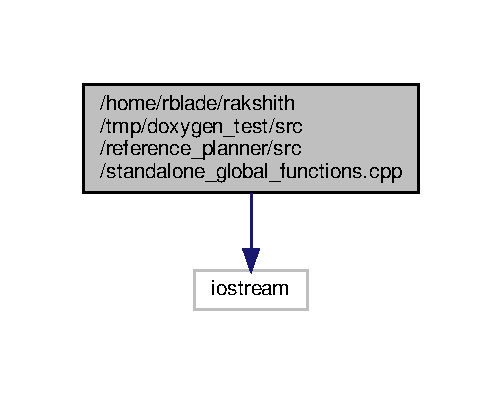
\includegraphics[width=241pt]{reference__planner_2src_2standalone__global__functions_8cpp__incl}
\end{center}
\end{figure}
\subsection*{Functions}
\begin{DoxyCompactItemize}
\item 
int \hyperlink{reference__planner_2src_2standalone__global__functions_8cpp_a7e16525f4cd8e93e798db81511a23c64}{ref\+\_\+plan} (int x, int y)
\begin{DoxyCompactList}\small\item\em ref\+\_\+planner function definition \end{DoxyCompactList}\item 
\mbox{\Hypertarget{reference__planner_2src_2standalone__global__functions_8cpp_ae66f6b31b5ad750f1fe042a706a4e3d4}\label{reference__planner_2src_2standalone__global__functions_8cpp_ae66f6b31b5ad750f1fe042a706a4e3d4}} 
int {\bfseries main} ()
\end{DoxyCompactItemize}


\subsection{Function Documentation}
\mbox{\Hypertarget{reference__planner_2src_2standalone__global__functions_8cpp_a7e16525f4cd8e93e798db81511a23c64}\label{reference__planner_2src_2standalone__global__functions_8cpp_a7e16525f4cd8e93e798db81511a23c64}} 
\index{reference\+\_\+planner/src/standalone\+\_\+global\+\_\+functions.\+cpp@{reference\+\_\+planner/src/standalone\+\_\+global\+\_\+functions.\+cpp}!ref\+\_\+plan@{ref\+\_\+plan}}
\index{ref\+\_\+plan@{ref\+\_\+plan}!reference\+\_\+planner/src/standalone\+\_\+global\+\_\+functions.\+cpp@{reference\+\_\+planner/src/standalone\+\_\+global\+\_\+functions.\+cpp}}
\subsubsection{\texorpdfstring{ref\+\_\+plan()}{ref\_plan()}}
{\footnotesize\ttfamily int ref\+\_\+plan (\begin{DoxyParamCaption}\item[{int}]{x,  }\item[{int}]{y }\end{DoxyParamCaption})}



ref\+\_\+planner function definition 


\begin{DoxyParams}{Parameters}
{\em x} & -\/ param1 \\
\hline
{\em y} & -\/ param2 ... text ... \\
\hline
\end{DoxyParams}
comment 1

comment 2 
%--- End generated contents ---

% Index
\backmatter
\newpage
\phantomsection
\clearemptydoublepage
\addcontentsline{toc}{chapter}{Index}
\printindex

\end{document}
